\documentclass[12pt]{article}
\usepackage[utf8]{inputenc}
\usepackage[a4paper,margin=1in]{geometry}
\usepackage{amsmath} 
\usepackage{amssymb}
\usepackage{graphicx}
\usepackage{float}
\usepackage{tabularx} 
\usepackage{caption}
\usepackage{subcaption}
\usepackage{array}
\usepackage{listings}
\usepackage{pythonhighlight}



\title{
    Department Of Aerospace Engineering,\\
    Indian Institute Of Technology Madras
    \begin{figure}[H]
        \centering
        
\includegraphics[width=8cm]{iitmlogo.png}
    \end{figure}
    \begin{center}
        \textbf{\\AS2101 : Introduction to Aerospace Engineering\\}
        Report 5 :Area under curve by various Quadrature Methods\\
    \end{center}
}
\author{
    Pranit Zope\\AE20B046
}
\date{October 7, 2021}

\begin{document}
\pagenumbering{gobble}
\maketitle
\newpage
\pagenumbering{arabic}
\tableofcontents 
\listoffigures

\newpage
\section{Aim}
Our aim is to find the area under the graph $y=sin(x)$ using the given methods of \textit{Quadrature}.
\begin{enumerate}
    \item Left-End Method
    \item Right-End Method
    \item Mid-Point Method
    \item Trapezoid Method
\end{enumerate}

\section{Theory}
We will now look at all the four methods here, explained in detail. But first, we need to understand what a riemann sum is
\subsection{Riemann Sum}
\begin{figure}[H]
    \centering
    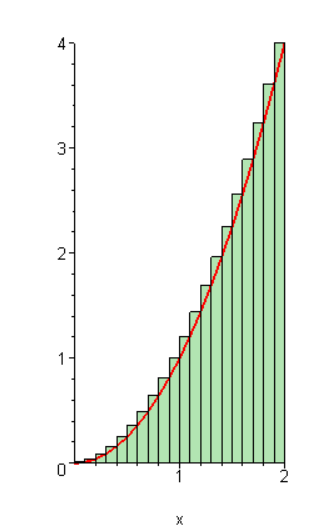
\includegraphics[width=4cm]{riemann.png}
    \caption{Riemann sum of the function $y=x^2$}
    \label{fig:rmn}
\end{figure}
Riemann Sum is basically a technique that allows us to calculate the area under functions by dividing the area into small rectangles of very small width, and then summing it up. Suppose you divide the area into recangles of width $dx$ each, the riemann sum will hence be :
\begin{equation*}
    \int^b_a f(x) = \sum f(x) \cdot dx
\end{equation*}

\subsection{Left-End Method}
In this method, we divide the rectangles into width $dx$ and height of the left end of the rectangle, that is equal to $f(x)$.
The illustrations depicts it more clearly.
\begin{figure}[H]
    \centering
    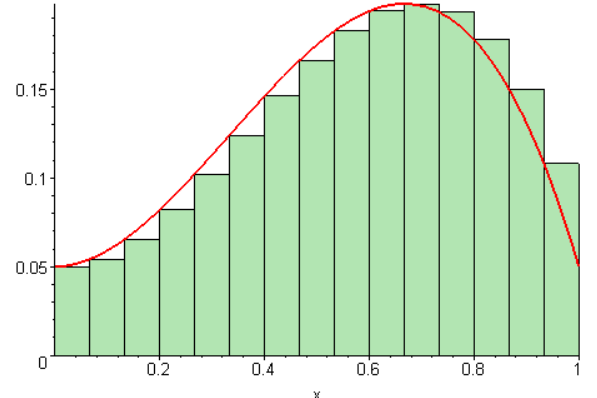
\includegraphics[width=6cm]{lefts.png}
    \caption{Left-End Method}
    \label{fig:lefts}
\end{figure}
\begin{equation}
    A=\sum_{n=0}^N f(x+ndx)\cdot dx
\end{equation}

\subsection{Right-End Method}
In this method, we divide the rectangles into width $dx$ and height of the right end of the rectangle, that is equal to $f(x+dx)$.
The illustrations depicts it more clearly.
\begin{figure}[H]
    \centering
    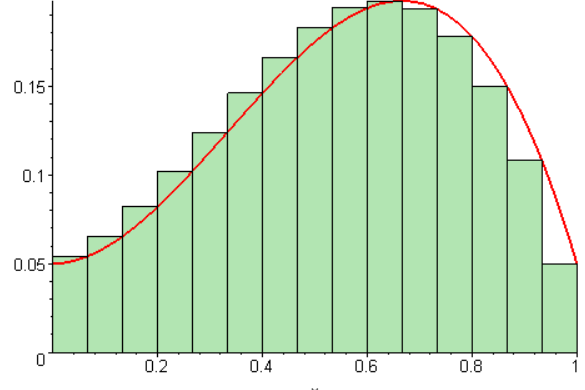
\includegraphics[width=6cm]{rights.png}
    \caption{Right-End Method}
    \label{fig:rights}
\end{figure}
\begin{equation}
    A=\sum_{n=0}^N f(x+(n+1)dx)\cdot dx
\end{equation}


\subsection{Mid-Point Method}
In this method, we divide the rectangles into width $dx$ and height of the midpoint of the rectangle, that is equal to $f(\frac{x+dx}{2})$.
The illustrations depicts it more clearly.
\begin{figure}[H]
    \centering
    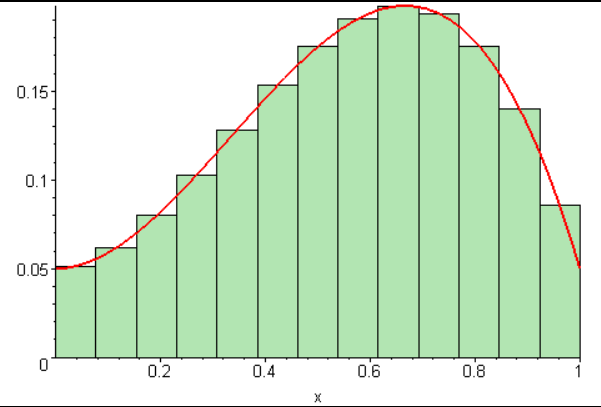
\includegraphics[width=6cm]{mids.png}
    \caption{Midpoint Method}
    \label{fig:mids}
\end{figure}
\begin{equation}
    A=\sum_{n=0}^N f(\frac{x+dx}{2})\cdot dx
\end{equation}


\subsection{Trapezoid Method}
In this method, we divide the trapezoids whose height is $dx$ and the two unequal edges are $f(x)$and$f(x+dx)$
The illustrations depicts it more clearly.
\begin{figure}[H]
    \centering
    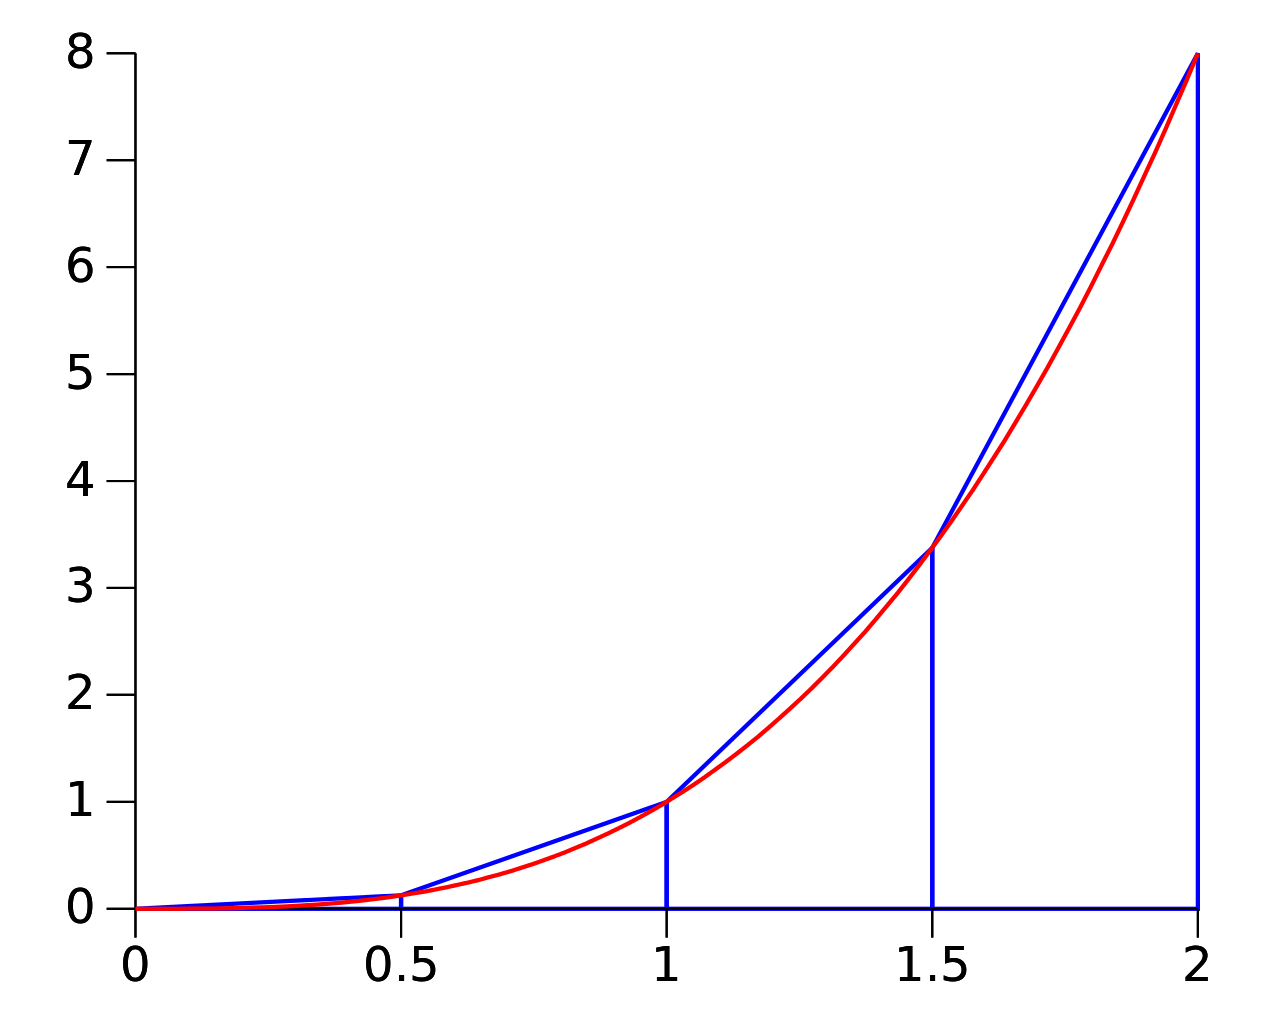
\includegraphics[width=6cm]{traps.png}
    \caption{Right-End Method}
    \label{fig:traps}
\end{figure}
\begin{equation}
    A=\sum_{n=0}^N \frac{f(x)+f(x+dx)}{2} \cdot dx
\end{equation}


\section{Plots}

\begin{figure}[H]
    \centering
    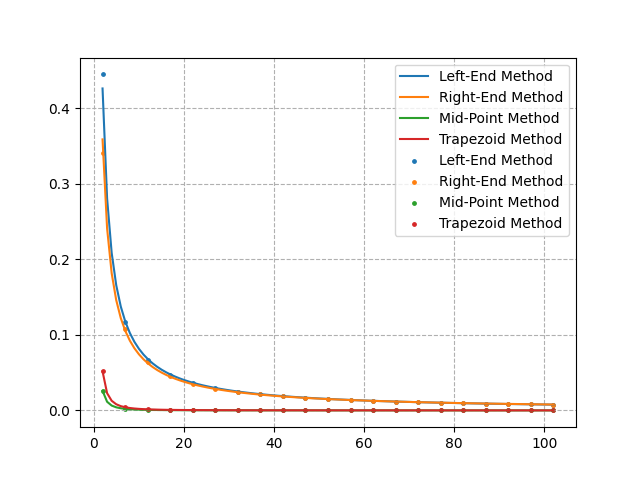
\includegraphics[width=13cm]{error4.png}
    \caption{Absolute Error for all methods}
\end{figure}

\begin{figure}[H]
    \centering
    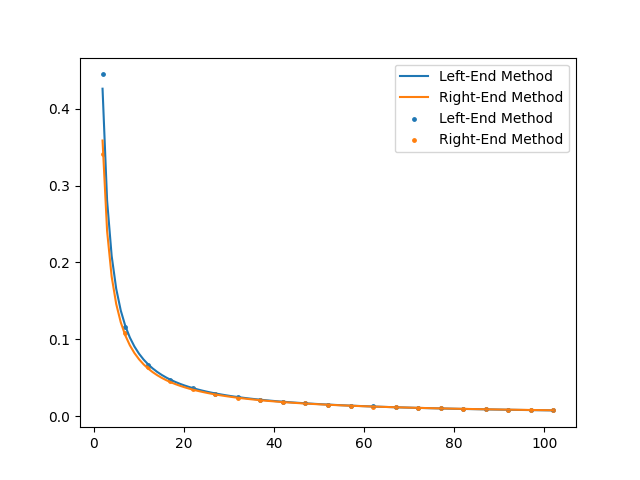
\includegraphics[width=13cm]{error_rl.png}
    \caption{A comparision of Rightend and Leftend Method}
\end{figure}

\begin{figure}[H]
    \centering
    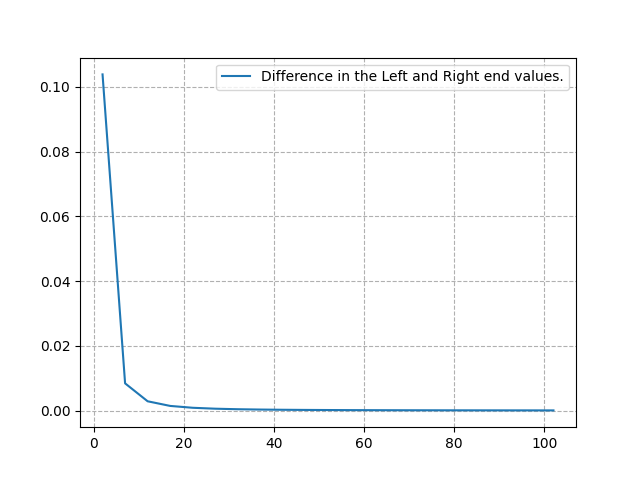
\includegraphics[width=13cm]{diff.png}
    \caption{Difference between Results of Right and Left Method}
\end{figure}

\begin{figure}[H]
    \centering
    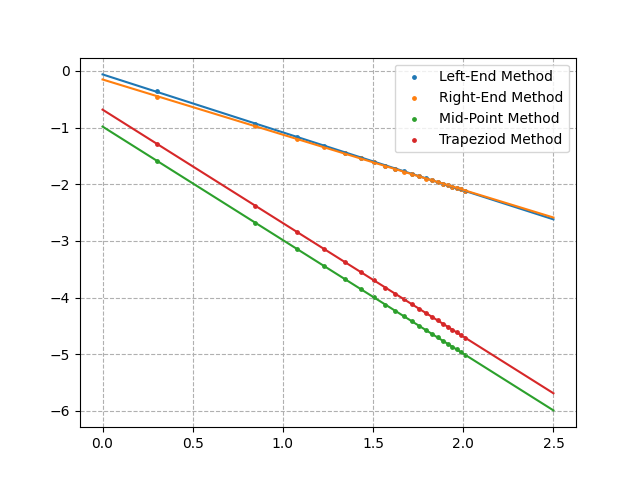
\includegraphics[width=13cm]{log4.png}
    \caption{Comparision of the 4 methods (Logarithm)}
\end{figure}

%%%%%%%%%%%%%%%%%%%%%%%%%%%%%%%%%%%%%%%%%%%%%%%%%%%
%%%%%%%%%%%%%%%%%%%%%%%%%%%%%%%%%%%%%%%%%%%%%%%%%%%
%%%%%%%%%%%%%%%%%%%%%%%%%%%%%%%%%%%%%%%%%%%%%%%%%%%
%%%%%%%%%%%%%%%%%%%%%%%%%%%%%%%%%%%%%%%%%%%%%%%%%%%

\begin{figure}[H]
    \centering
    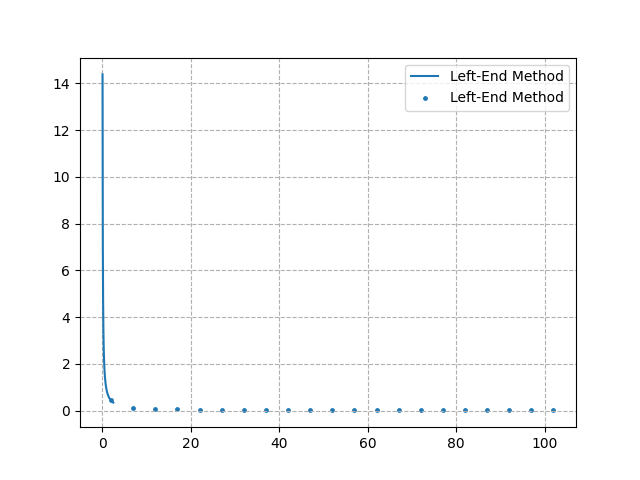
\includegraphics[width=13cm]{left.png}
    \caption{Left-End Method}
\end{figure}


\begin{figure}[H]
    \centering
    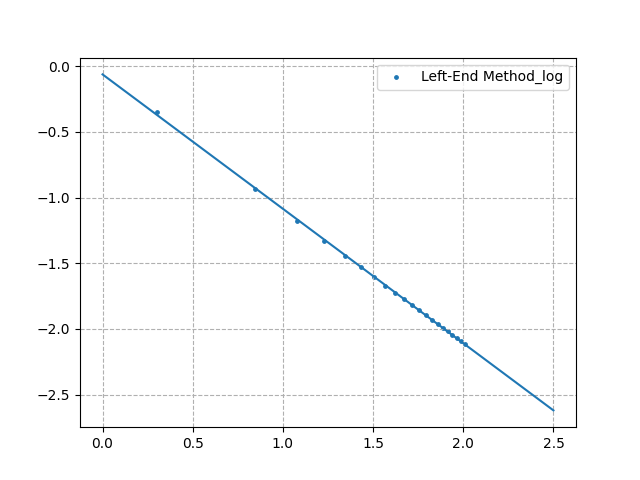
\includegraphics[width=13cm]{leftlog.png}
    \caption{Left-End Method(Logarithm)}
\end{figure}


\begin{figure}[H]
    \centering
    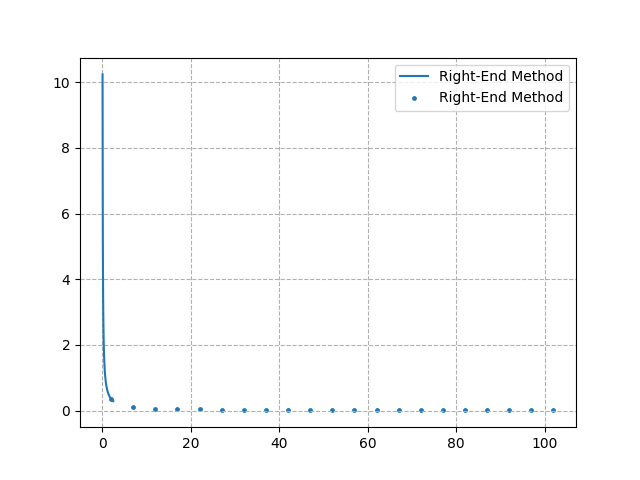
\includegraphics[width=13cm]{right.png}
    \caption{Right-End Method}
\end{figure}

\begin{figure}[H]
    \centering
    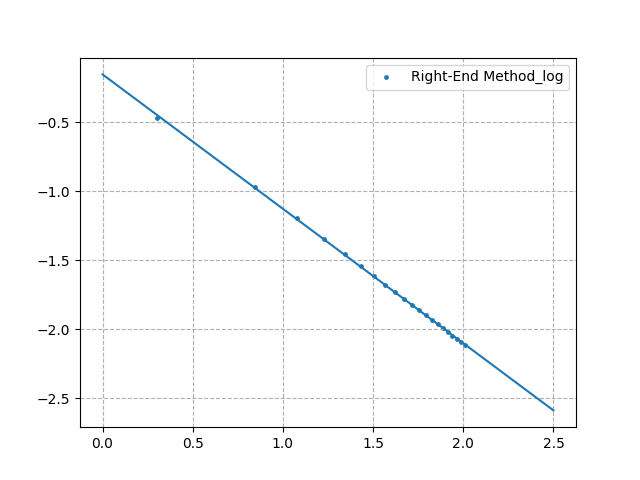
\includegraphics[width=13cm]{rightlog.png}
    \caption{Right-End Method (Logarithm)}
\end{figure}

\begin{figure}[H]
    \centering
    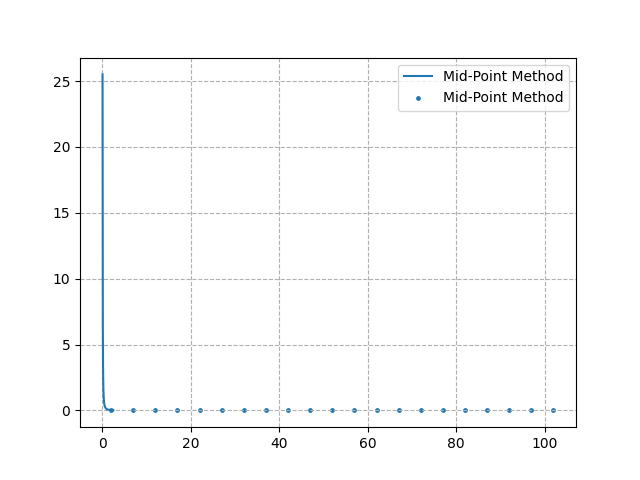
\includegraphics[width=13cm]{midpt.png}
    \caption{Midpoint Method}
\end{figure}

\begin{figure}[H]
    \centering
    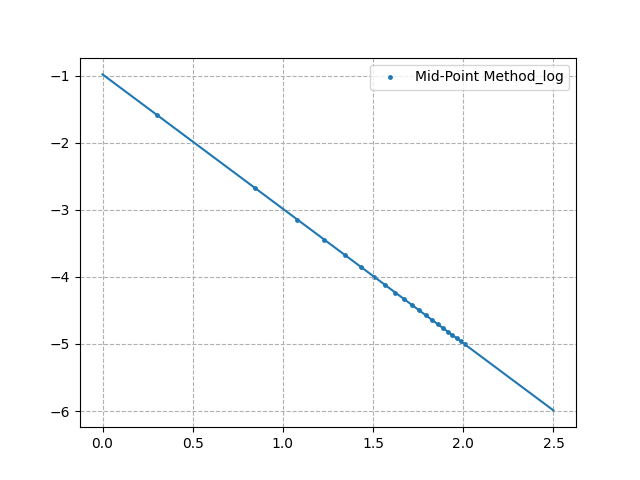
\includegraphics[width=13cm]{midlog.png}
    \caption{Midpoint Method (Logarithm)}
\end{figure}

\begin{figure}[H]
    \centering
    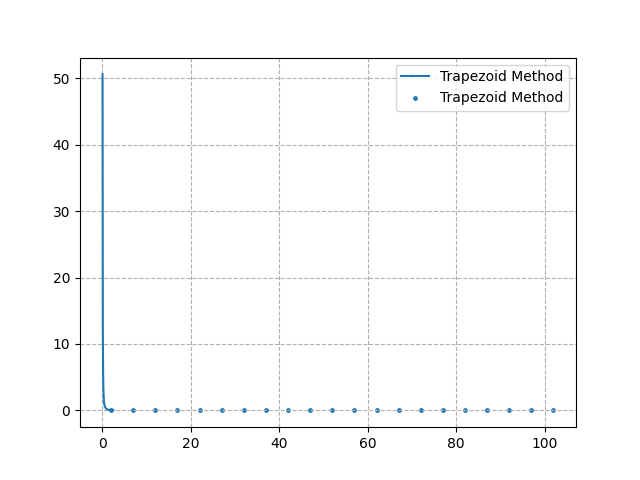
\includegraphics[width=13cm]{trap.png}
    \caption{Trapezoid Method}
\end{figure}

\begin{figure}[H]
    \centering
    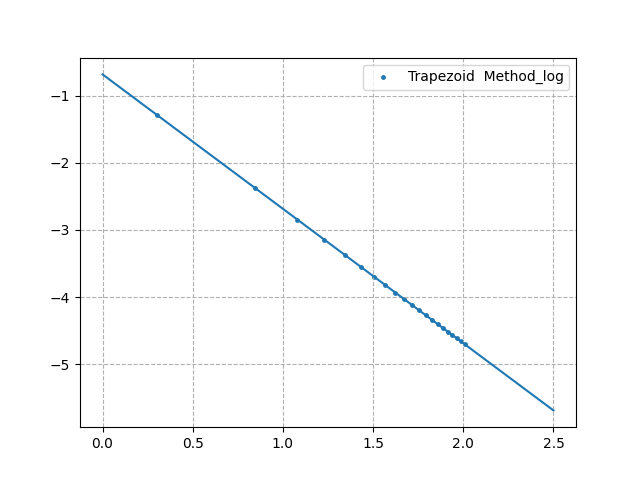
\includegraphics[width=13cm]{traplog.png}
    \caption{Trapezoid Method (Logarithm)}
\end{figure}

\newpage
\appendix
\addcontentsline{toc}{section}{Appendix}

\section{Python Code containing Different Methods of Quadrature}
\begin{python}
#!/usr/bin/env/python3.9
# Pranit Zope
# AE20B046
# Task 05 : Integrals using Quadrature
# File containing the fucntions of various methods used

import numpy as np

def leftep(n):
    dx=(np.pi/2)/n
    area=0
    x=0
    for i in range(n):
        area=area+np.sin(x)*dx
        x=x+dx
    return area

def rightep(n):
    dx=(np.pi/2)/n
    area=0
    x=dx
    for i in range(n):
        area=area+np.sin(x)*dx
        x=x+dx
    return area

def midpt(n):
    dx=(np.pi/2)/n
    area=0
    x=dx/2
    for i in range(n):
        area=area+np.sin(x)*dx
        x=x+dx
    return area

def trapezoid(n):
    dx=(np.pi/2)/n
    area=0
    x=0
    for i in range(n):
        temp=((np.sin(x)+np.sin(x+dx))/2)*dx
        area=area+temp
        x=x+dx
    return area

\end{python}
\section{Python Code for Linear Regression}
\begin{python}
#!/usr/bin/env/python3.9
# Pranit Zope
# AE20B046
# Task 05 : Integrals using Quadrature
# File containing the fucntions used for regression (directly taken from Task02)

import numpy as np
from matplotlib import pyplot as plt



def determinant(m):
    det=m[0][0]*m[1][1]-m[0][1]*m[1][0]
    return det

def inverse(m):
    inv=np.zeros((2,2))
    inv[0][0]=m[1][1]/determinant(m)
    inv[0][1]=-1*(m[0][1]/determinant(m))
    inv[1][0]=-1*(m[1][0]/determinant(m))
    inv[1][1]=(m[0][0]/determinant(m))
    return inv

def transpose(m,size):
    temp=np.ones((2,size))
    for i in range(0,size):
        temp[1][i]=m[i][1]
    return temp


def prod(AT,a,b,A,c,d):
    if(b==c):
        temp=np.zeros((a,d))
        for i in range(a):
            for j in range(d):
                sum=0
                for k in range(b):
                    sum=sum+AT[i][k]*A[k][j]
                temp[i][j]=sum
        return temp

def curve(A1,B1):             
    size=len(A1)
    A=np.ones((size,2))
    for i in range(0,size):
        A[i][1]=np.log10(A1[i])
    
    B=np.zeros((size,2))
    for i in range(size):
        B[i][0]=np.log10(B1[i])
    

    AT=transpose(A,size)
    AT_A=prod(AT,2,size,A,size,2)
    AT_A_inv=inverse(AT_A)
    AT_B=prod(AT,2,size,B,size,1)
    sol=prod(AT_A_inv,2,2,AT_B,2,1)
   
    return sol


def bfline(A1,B1):
    size=len(A1)
    A=np.ones((size,2))
    for i in range(0,size):
        A[i][1]=A1[i]
    B=np.zeros((size,2))
    for i in range(size):
        B[i][0]=B1[i]
    AT=transpose(A,size)
    AT_A=prod(AT,2,size,A,size,2)
    AT_A_inv=inverse(AT_A)
    AT_B=prod(AT,2,size,B,size,1)
    sol=prod(AT_A_inv,2,2,AT_B,2,1)

    return sol
\end{python}
\section{Python Code : Main file and plotting}
\begin{python}
#!/usr/bin/env/python3.9
# Pranit Zope
# AE20B046
# Task 05 : Integrals using Quadrature
# Main file

import numpy as np
from matplotlib import pyplot as plt
import methods
import regression

Area=1  #we know that area under sine curve is one

total=[]
k=2
while(k<103):
    total.append(k)
    k=k+5

left=[]
right=[]
mid=[]
trapez=[]

for i in total:
    left.append(abs(Area-methods.leftep(i)))
    right.append(abs(Area-methods.rightep(i)))
    mid.append(abs(Area-methods.midpt(i)))
    trapez.append(abs(Area-methods.trapezoid(i)))

x=np.linspace(2,102,100)

plt.figure()
plt.grid(linestyle='--')


##############  Graph 1 : Absolute error for all methods #################

plt.scatter(total,left,label='Left-End Method',s=6)
b=regression.curve(total,left)[1]
a=10**regression.curve(total,left)[0]
plt.plot(x,a*(x**b),label='Left-End Method')

plt.scatter(total,right,label='Right-End Method',s=6)
b=regression.curve(total,right)[1]
a=10**regression.curve(total,right)[0]
plt.plot(x,a*(x**b),label='Right-End Method')

plt.scatter(total,mid,label='Mid-Point Method',s=6)
b=regression.curve(total,mid)[1]
a=10**regression.curve(total,mid)[0]
plt.plot(x,a*(x**b),label='Mid-Point Method')

plt.scatter(total,trapez,label='Trapezoid Method',s=6)
b=regression.curve(total,trapez)[1]
a=10**regression.curve(total,trapez)[0]
plt.plot(x,a*(x**b),label='Trapezoid Method')
plt.legend()
plt.show()
plt.savefig('Error4.png')
plt.clf()

##############  Graph 2 : Comparision of right and left method #################

plt.scatter(total,left,label='Left-End Method',s=6)
b=regression.curve(total,left)[1]
a=10**regression.curve(total,left)[0]
plt.plot(x,a*(x**b),label='Left-End Method')

plt.scatter(total,right,label='Right-End Method',s=6)
b=regression.curve(total,right)[1]
a=10**regression.curve(total,right)[0]
plt.plot(x,a*(x**b),label='Right-End Method')
plt.legend()
plt.show()
plt.savefig('ErrorRL.png')
plt.clf()

################

total_log=[]; t=2
while(t<103):
    total_log.append(np.log10(t))
    t=t+5

size=len(left)

leftlog=np.zeros(size)
rightlog=np.zeros(size)
midlog=np.zeros(size)
trapezlog=np.zeros(size)

for j in range(size):
    leftlog[j]=np.log10(left[j])
    rightlog[j]=np.log10(right[j])
    midlog[j]=np.log10(mid[j])
    trapezlog[j]=np.log10(trapez[j])



plt.grid(linestyle='--')

x=np.linspace(0,2.5,40)

##############  Graph 3 : Logarithms of all methods #################

plt.scatter(total_log,leftlog,label='Left-End Method',s=6)
m=regression.bfline(total_log,leftlog)[1]
c=regression.bfline(total_log,leftlog)[0]
plt.plot(x,m*x+c)

plt.scatter(total_log,rightlog,label='Right-End Method',s=6)
m=regression.bfline(total_log,rightlog)[1]
c=regression.bfline(total_log,rightlog)[0]
plt.plot(x,m*x+c)

plt.scatter(total_log,midlog,label='Mid-Point Method',s=6)
m=regression.bfline(total_log,midlog)[1]
c=regression.bfline(total_log,midlog)[0]
plt.plot(x,m*x+c)

plt.scatter(total_log,trapezlog,label='Trapeziod Method',s=6)
m=regression.bfline(total_log,trapezlog)[1]
c=regression.bfline(total_log,trapezlog)[0]
plt.plot(x,m*x+c)

plt.legend()
plt.show()
plt.savefig('Error4log.png')
plt.clf()


#####################

diff=np.zeros(size)
for i in range(size):
    diff[i]=(left[i]-right[i])

plt.grid(linestyle='--')
plt.plot(total,diff,label='Difference in the Left and Right end values.')
plt.legend()
plt.show()
plt.savefig('diff_rl.png')
plt.clf()

##############  Later graphs : plotting all methods  and their logarithms #################

def normalplot(data,lbl):
    plt.grid(linestyle='--')
    plt.ylim(-5,50)
    plt.scatter(total,data,label=lbl,s=6)
    b=regression.curve(total,data)[1]
    a=10**regression.curve(total,data)[0]
    plt.plot(x,a*(x**b),label=lbl)
    plt.legend()
    plt.show()
    plt.savefig(lbl+".png")
    plt.clf()


def logplot(data,lbl):
    plt.grid(linestyle='--')
    plt.scatter(total_log,data,label=lbl,s=6)
    m=regression.bfline(total_log,data)[1]
    c=regression.bfline(total_log,data)[0]
    plt.plot(x,m*x+c)
    plt.legend()
    plt.show()
    plt.savefig(lbl+".png")
    plt.clf()


normalplot(left,"Left-End Method")
normalplot(right,"Right-End Method")
normalplot(mid,"Mid-Point Method")
normalplot(trapez,"Trapezoid Method")

logplot(leftlog,"Left-End Method_log")
logplot(rightlog,"Right-End Method_log")
logplot(midlog,"Mid-Point Method_log")
logplot(trapezlog,"Trapezoid  Method_log")
\end{python}
\end{document}
